\documentclass{article}
\usepackage{graphicx,ulem} 
\usepackage{color}
\usepackage{amsfonts,amsmath}
\usepackage{amsthm}
\usepackage{empheq}
\usepackage{mathtools}
\usepackage{multirow}
%\usepackage{tikz}
\usepackage{titlesec}
\usepackage{caption}
%\usepackage{lscape}
\usepackage{graphicx}
\captionsetup{justification=justified}
\usepackage[toc,page]{appendix}
\usepackage{hyperref}
\usepackage{subcaption}
\usepackage{pdftricks}
\usepackage{xcolor}
\begin{psinputs}
\usepackage{amsfonts,amsmath}
	\usepackage{pstricks-add}
   \usepackage{pstricks, pst-node}
   \usepackage{multido}
   \newcommand{\lfw}{\lambda_{F}}
\end{psinputs}

\textheight240mm \voffset-23mm \textwidth160mm \hoffset-20mm

 \graphicspath{{./Images/}{../Schema}{./Images/HT1/}}
%\graphicspath{{Figures}}
\setcounter{secnumdepth}{4}
\titleformat{\paragraph}
{\normalfont\normalsize\bfseries}{\theparagraph}{1em}{}
\titlespacing*{\paragraph}
{0pt}{3.25ex plus 1ex minus .2ex}{1.5ex plus .2ex}

\newcommand{\lfd}{\lambda_{F, D}}
\newcommand{\lfw}{\lambda_{F}}
\newcommand{\Kfa}{K_{F,\alpha}}
\newcommand{\cI}{\mathcal{I}}
\newcommand{\mW}{\tilde{m}_W}
\newcommand{\mD}{\tilde{m}_D}
\newcommand{\vb}{\mathbf{b}}

\newcommand{\marc}[1]{\textcolor{teal}{#1}}
\newcommand{\YD}[1]{\textcolor{magenta}{#1}}
\newcommand{\VY}[1]{\textcolor{blue}{#1}}
\newcommand{\vdeux}[1]{\textcolor{orange}{#1}}

\DeclareMathOperator{\Tr}{Tr}
\newtheorem{theorem}{Theorem}
\newtheorem{prop}[theorem]{Proposition}
\theoremstyle{definition}
\newtheorem{definition}[theorem]{Definition}
\theoremstyle{remark}
\newtheorem{remark}[theorem]{Remark}
\newtheorem{cor}[theorem]{Corollary}
\newcommand*\phantomrel[1]{\mathrel{\phantom{#1}}}

\title{Impact of anthropisation and over-hunting on the coexistence between humans and wildlife.}
\author{Yves Dumont, Marc Hétier and Valaire Yatat-Djeumen}
\begin{document}

\maketitle

\begin{prop} \label{prop: equivalentSystem}
We consider the following system:
\begin{equation}
\def\arraystretch{2}
\left\{ \begin{array}{l}
\dfrac{dh_D}{dt}= \cI + e\lfw h_W f_W + (f_D - \mu_D) h_D - m_D h_D - m_W h_W, \\
\dfrac{df_W}{dt} = (1-\alpha)(1 - \beta h_W) r_F \left(1 + \dfrac{f_W}{K_F(1-\alpha)} \right) f_W + \lfw f_W h_W, \\
\dfrac{dh_W}{dt}= -m_D h_D - m_W h_W. 
\end{array} \right.
\label{equation:hdfwhw}
\end{equation}
We note $y_{eq} = (h_D, f_W, h_W)$ the equivalent variables and $f_{eq}(y_{eq})$ the right hand side of \eqref{equation:hdfwhw}. This equivalent system is irreducible and dissipative, and
\begin{itemize}
\item if $\lfw - (1-\alpha)\beta r_F \geq 0$, it is competitive on $\Big\{(h_D, f_W, h_W) | 0 \leq h_D, f_W  \leq 0, h_W \leq 0 \Big\}$,
\item if $\lfw - (1-\alpha)\beta r_F < 0$, it is competitive on $\Big\{(h_D, f_W, h_W) | 0 \leq h_D, f_W \leq K_F\big(\dfrac{\lfw}{\beta r_F}-(1-\alpha)\big), h_W \leq 0 \Big\}$ 
\end{itemize}

Moreover, we know that it defines a dynamical system on 
$$
\Omega_{eq} 
 = \Big\{\Big(h_D, f_W, h_W \Big) \in \mathbb{R_+} \times (\mathbb{R_-})^2 \Big|h_D - ef_W \leq S^{max}, -F_W^{max} \leq f_W \leq 0, -H_W^{max} \leq h_W \leq 0 \Big\}
 $$
 where
$$
S^{max} = \dfrac{\cI + \left( \mu_D - f_D   +  \dfrac{(1-\alpha)r_F}{4}\right)e(1-\alpha)K_F}{  \Big(\mu_D -f_D - \dfrac{er_F (1-\alpha)^2K_F m}{4} \beta\Big)} ,
\quad
F_W^{max} = (1-\alpha)K_F,
\quad
H_W^{max} = \dfrac{m_D}{m_W} S^{max}.
$$
\end{prop}

\begin{prop}
The following results hold true:
\begin{itemize}
\item When $\cI = 0$, the system \eqref{equation:hdfwhw} admits a fauna only equilibrium $EE^{f_W} = \Big(0,-K_F(1-\alpha), 0 \Big)$ which is LAS if $\mathcal{N}_{\cI = 0} := \dfrac{m e \lfw (1-\alpha)K_F}{\mu_D - f_D} < 1$.
\item When $\cI > 0$, the system \eqref{equation:hdfwhw} admits a human only equilibrium $EE^{h} = \Big(\dfrac{\cI}{\mu_D - f_D}, 0, -\dfrac{m_D}{m_W}\dfrac{\cI}{\mu_D - f_D} \Big)$ which is LAS if $\mathcal{N}_{\cI > 0} := \dfrac{r_F(1-\alpha)\Big({\dfrac{\mu_D - f_D}{m\cI}+\beta\Big)}}{\lfw} < 1$.
\end{itemize}
\end{prop}
\newpage
\begin{remark}
Straightforward computations give the black notations on the following graphic. \textcolor{red}{Red notations} concern stability of\textcolor{red}{ $EE^{f_W}$}, \textcolor{blue}{blue ones} concern stability of \textcolor{blue}{$EE^{h}$}.
\begin{figure}[!ht]
\centering
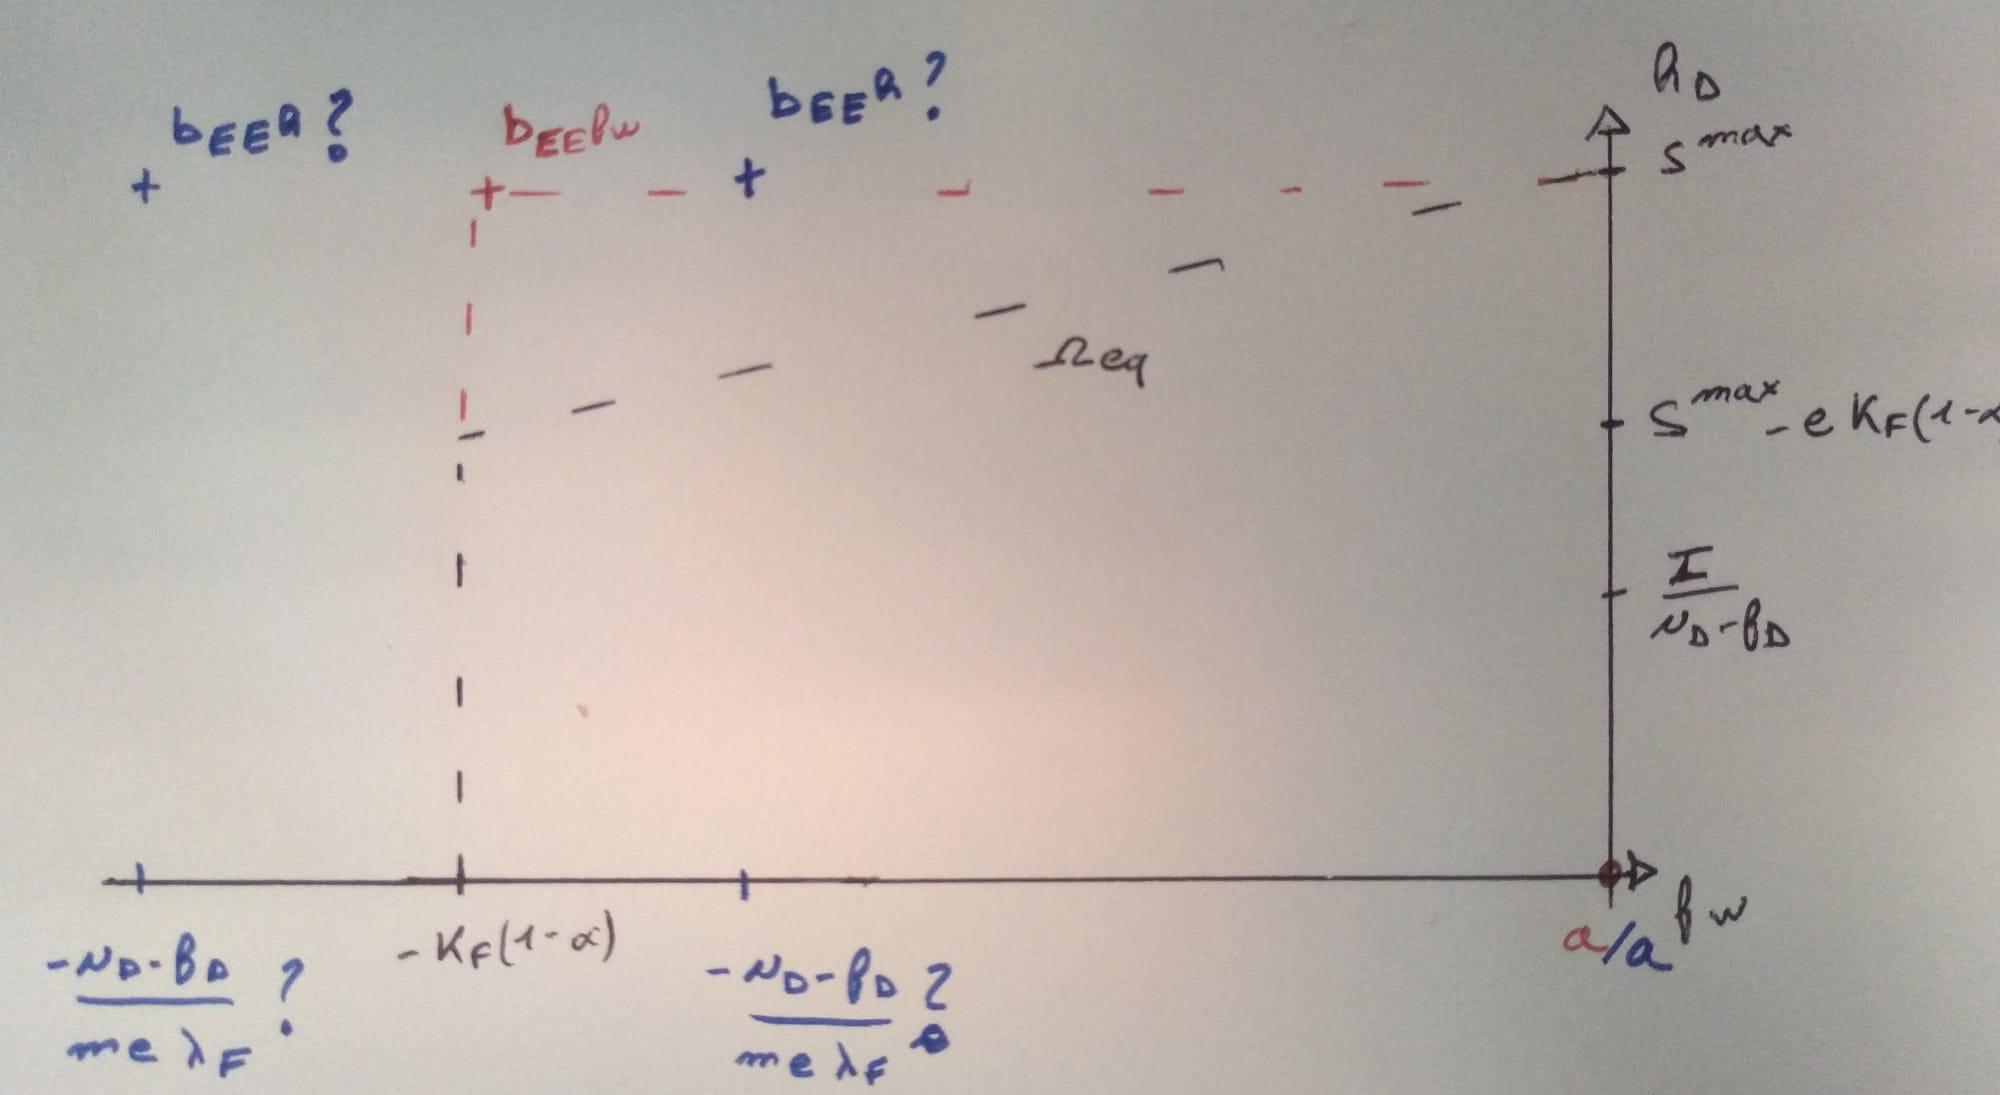
\includegraphics[width=1\textwidth]{OmegaEq.jpeg}
\end{figure}

\end{remark}
Given this, the inequalities between vectors of $\mathbb{R}^3$ are considered in the following sense:
$$
a \leq b \Leftrightarrow \left\lbrace \begin{array}{l} 
a_1 \leq b_1 \\ -a_2 \leq - b_2 \\ -a_3 \leq - b_3
\end{array} \right.
$$
In addition, we introduce the notations: $a < b \Leftrightarrow a \leq b$ and $a\neq b$; and $[a,b] = \lbrace x \in \mathbb{R}^3 | a \leq x \leq b \rbrace$

We also recall the following theorem:
\begin{theorem} \label{theorem: monotone GAS} Theorem 3 of \cite{anguelov_monotone_2010}.

Let $\dfrac{dy}{dt} = f(y)$ be monotone (and in particular competitive) and let $a,b \in \mathcal{D}$ such that $a <b$, $[a, b] \subset \mathcal{D}$ and $f(b) \leq \mathbf{0} \leq f(a)$. Then the system defines a positive dynamical system on $[a, b] $. Moreover, if $[a, b] $ contains a unique equilibrium then it is GAS on $[a, b] $.
\end{theorem}

We will use it to prove the following two propositions. 

\begin{prop}
When $\cI = 0$ and when $\mathcal{N}_{I=0} \leq 1$, the fauna only equilibrium $EE^{F_W}$ is GAS on $\Omega_{eq}$
\end{prop}


\begin{proof} 
We search for $\mathbf{b} = (h_D, f_W, h_W)$ such that $EE^{f_W} \in \Big[\mathbf{0}, \mathbf{b} \Big]$ and $f_{eq}(\vb) \leq 0$.
Since $EE^{f_W}_2 = -K_F(1-\alpha)$, and given $\Omega_{eq}$, we will take $b_2 = -K_F(1-\alpha)$.

This gives $f_{eq, 2}(\mathbf{b}) = -\lfw K_F(1-\alpha) h_W$ and therefore $-f_{eq, 2}(\mathbf{b}) \leq 0$ for all $h_W \leq 0$, which is what we want.

We also have $f_{eq,3}(\mathbf{b}) = -m_D h_D - m_W h_W$ and we want $-f_{eq,3}(\mathbf{b}) \leq 0$. This is possible only if 
\begin{equation}
h_W \leq -\dfrac{m_D}{m_W}h_D.
\end{equation}

Now we compute $f_{eq,1}(\mathbf{b})$; we want it negative:
\begin{align*}
f_{eq,1}(\mathbf{b}) &= -\Big(e\lfw K_F(1-\alpha) + m_W\Big)h_W - \Big(\mu_D - f_D + m_D\Big) h_D \\
& \leq -\Big((\mu_D - f_D)\dfrac{m_W}{m_D} + m_W\Big)h_W - \Big(\mu_D - f_D + m_D\Big) h_D \quad \text{using $N_{I= 0} = \dfrac{m e \lfw (1-\alpha)K_F}{\mu_D - f_D} \leq 1$} \\
& \leq - \Big(\mu_D - f_D + m_D\Big)( h_D + \dfrac{m_W}{m_D}h_W )
\end{align*}
This last quantity is negative only if 

\begin{equation} h_W \geq - \dfrac{m_D}{m_W}h_D. \end{equation}
Given (2) and (3), we have to take $b_3 = - \dfrac{m_D}{m_W}h_D$. 

We have no constraint on $b_1$, and therefore we can take $b_1 = S^{max}$ so that $\Omega_{eq} \subset [\mathbf{0}, \mathbf{b}]$

\end{proof}

\begin{remark}
When $\lfw - (1-\alpha)\beta r_F < 0$, the system is not competitive on $\Omega_{eq}$, but only in $\Omega_1 = \Big\{(h_D, f_W, h_W) | 0 \leq h_D, f_W \leq K_F\big(\dfrac{\lfw}{\beta r_F}-(1-\alpha)\big), h_W \leq 0 \Big\}$. The vector $a = \mathbf{0}$ does not lay in this region, and should be replace in the previous proof by $a = \Big(0, K_F\big(\dfrac{\lfw}{\beta r_F}-(1-\alpha)\big), 0)$ which still verify the theorem hypothesis ($a \leq EE^{f_W} \leq b$ and $f_{eq}(a) \geq 0$). Since $\Omega_1$ is an absorbing set, the conclusion remains the same.
\end{remark}

Now, we look for the global stability of the human only equilibrium.

\begin{prop}
When $\cI > 0$ and when $\mathcal{N}_{I>0} \leq 1$, the following holds true.

For each $f_W$ such that $-\dfrac{\mu_D-f_D}{me \lfw} < f_W \leq 0$ and $\dfrac{I}{\mu_D - f_D + me \lfw f_W} \leq h_D$ the human only equilibrium $EE^{h}$ is GAS on $[\mathbf{0}, \Big(S^{max}, f_W, - m S^{max}\Big)]$
\end{prop}

\begin{proof}
We search for a vector $\vb=(h_D, f_W, h_W)$ such that $EE^{h} \leq \vb$ and $f_{eq}(\vb) \leq 0$. The first inequality gives $\dfrac{\cI}{\mu_D - f_D} \leq h_D$ and $h_W \leq - \dfrac{m_D}{m_W}\dfrac{\cI}{\mu_D - f_D}$.

We have $f_{eq,3}(\vb) =-m_D h_D - m_W h_W$ and we want $-f_{eq,3}(\mathbf{b}) \leq 0$. This is possible only if 
\begin{equation}
h_W \leq -\dfrac{m_D}{m_W}h_D.
\end{equation}
We have:
\begin{align*}
f_{eq, 2}(\vb) &= \left(r_F(1-\alpha) (1-\beta h_W) \left(1 + \dfrac{f_W}{K_F(1-\alpha)}\right) + \lfw h_W \right) f_W \\
f_{eq, 2}(\vb) &= \left(r_F(1-\alpha) \dfrac{(1-\beta h_W)}{\lfw h_W} + 1  + r_F(1-\alpha) \dfrac{(1-\beta h_W)}{\lfw h_W} \dfrac{f_W}{K_F(1-\alpha)} \right) \lfw h_W f_W
\end{align*}

Since $$\mathcal{N}_{I>0} = r_F(1-\alpha) \dfrac{1 + \beta m \dfrac{\cI}{\mu_D - f_D}}{\lfw m \dfrac{\cI}{\mu_D - f_D}} \leq 1$$

we obtain that for all $f_w \leq 0$ and $h_W \leq -\dfrac{m_D}{m_W}h_D \leq -\dfrac{m_D}{m_W} \dfrac{\cI}{\mu_D - f_D}$
$$
0 \leq f_{eq, 2}(\vb)
$$
is true without more constraints on $f_W$ or $h_W$.

Finally, we compute $f_{eq, 1}(\vb)$:

\begin{align*}
f_{eq, 1}(\vb) = \cI - (\mu_D - f_D)h_D -m_Dh_D - m_W h_W + e \lfw f_W h_W
\end{align*}
We want it negative. We have $\cI - (\mu_D - f_D) h_D \leq 0$ but $0 \leq e \lfw f_W h_W$ and $0 \leq -m_Dh_D - m_W h_W = f_{eq, 3}(\vb)$ (because of (4)). Therefore we choose $h_W = - \dfrac{m_D}{m_W}h_D$. This leads to:
\begin{align*}
f_{eq, 1}(\vb) = \cI - (\mu_D - f_D + em \lfw f_W)h_D.
\end{align*}
Since $0 \leq h_D$, $f_{eq, 1}(\vb)$ can be negative only if $0 < (\mu_D - f_D + em \lfw f_W)$ that is $- \dfrac{\mu_D - f_D}{me \lfw} < f_W$ and if $\dfrac{I}{\mu_D - f_D + me \lfw f_W} \leq h_D.$

Therefore, for each $f_W$ such that $- \dfrac{\mu_D - f_D}{me \lfw} < f_W \leq 0$, we can choose $h_D = \max(S^{max}, 
\dfrac{I}{\mu_D - f_D + me \lfw f_W})$ and $h_W = -\dfrac{m_D}{m_W}h_W$, and $\vb = (h_D, f_W, h_W)$. The previous computations show that $EE^{h}$ is GAS on $[\mathbf{0}, \vb]$ and therefore on $[\mathbf{0}, (S^{max}, f_W, \dfrac{-m_D}{m_W}S^{max})]$.
\end{proof}



\end{document}
